\chapter{Thick--Client VS Web--Browser--based
	Software--System Architecture}


\begin{table*}[!htbp]
\centering
\resizebox{\textwidth}{!}{%to fit the table within the text width
\begin{tabular}{cccc} 

\multicolumn{1}{c}{}										&
Thick--client application \mycheckmark{yerothColorBlue}	& 
Web--browser--based application								\\ \hline

business code								&
		\yerothrouge{all computers}			&						
		\yerothvert{application server}		\\ \hline
		
co--related software--systems		&
		\yerothvert{$1$ (DBMS)}		&						
		\yerothrouge{at least $3$ (DBMS, web~/~application server)}	\\ \hline
				
user interface											&
		\yerothvert{all computers (\thickclient gui)}	&						
		\yerothvert{all computers (web--browser)}		\\ \hline		
		
number of logical layers									&
		\yerothvert{$2$ (client and data)}					&						
		\yerothrouge{$4$ (client, presentation, logic, and data)}\\ \hline
				
rapid prototyping (\wy tools)		&
		\yerothvert{yes}			&						
		\yerothrouge{very limited}	\\ \hline				
				
software security vulnerability										&
		\yerothvert{low ($1$ programming language)}		&					
		\yerothrouge{high (\emph{several} programming languages)}	\\ 
\end{tabular}}
\caption{Thick--client application VS Web--browser--based application.\\}
\label{tab:thickclient-application-againts-webbrowserbased-application}
\end{table*}

\begin{center}
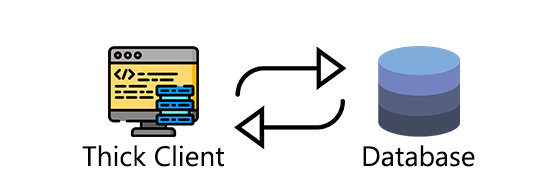
\includegraphics[scale=0.52]{images/yeroth-thickclient-application-two-tier-architecture.png}
\captionof{figure}{$2$--layers logical 
architecture of \thickclient software--system 
(copied from \cite{securityboulevarddotcom:2020}).}
\label{fig:yeroth-thickclient-application-two-tier-architecture}
\end{center}

Figure~\ref{fig:yeroth-thickclient-application-two-tier-architecture}
illustrates an example of a \thickclient
software--system with a $2$--layers
logical architecture.

\begin{center}
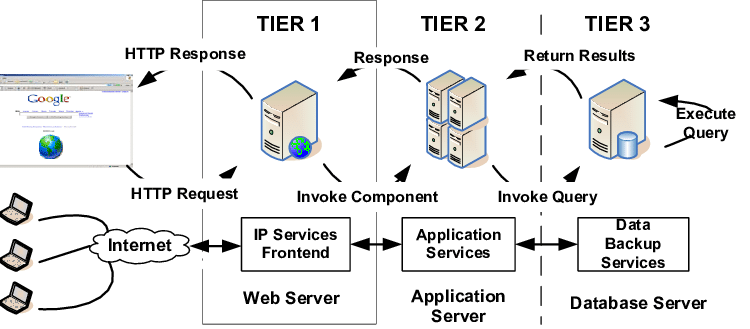
\includegraphics[scale=0.39]{images/yeroth-three-tier-architecture.png}
\captionof{figure}{$4$--layers logical architecture
of \webbrowserbased software--system
(copied from \cite{trevor:2006}).}
\label{fig:yeroth-three-tier-architecture}
\end{center}

Figure~\ref{fig:yeroth-three-tier-architecture}
illustrates an example of a \webbrowserbased
software--system with a $3$--layers
logical architecture.

Table~\ref{tab:thickclient-application-againts-webbrowserbased-application}
compares \thickclient software--systems against
\webbrowserbased software--systems.